\newgeometry{left=2cm,right=1cm,top=1cm,bottom=1cm,includefoot,heightrounded}

\section{Задача, зависящая от времени}
\label{timeDependent}

Пусть дано \textbf{гиперболическое} уравнение
\begin{equation}
\label{hyperbolicEqn}
	\chi \, \ddot{u} + \sigma \, \dot{u} - \nabla \cdot (a \, \nabla u) = f, \quad \vect{x} \in \Omega, \quad t \in \left[ t_0, \, t_l \right],
\end{equation}
с краевыми условиями~(\ref{BCs}) и начальными условиями
\begin{subequations}
\label{ICs}
	\begin{align}
		u(\vect{x}, t_0) &= u_0(\vect{x}), \\
		\dot{u}(\vect{x}, t_0) &= v_0(\vect{x}).
	\end{align}
\end{subequations}

Отличия от~(\ref{eqn}~--~\ref{BCs}): здесь через «\,$\dot{}$\,» обозначена производная по времени $t$, входные параметры $\chi = \chi(\vect{x})$, $\sigma = \sigma(\vect{x})$ и $a = a(\vect{x})$ есть функции пространства, а $\kappa = \kappa(\vect{x}, \, t)$, $g_D = g_D(\vect{x}, \, t)$ и $g_N = g_N(\vect{x}, \, t)$ --- функции пространства и времени.\\
$u_0$ есть начальное положение, $v_0$ --- начальная скорость.

Через $\left[ t_0, \, t_l \right] \subset \left[ 0, \infty \right) $ обозначен временной сегмент, в котором нужно найти решение $u = u(\textbf{x}, \, t)$, удовлетворяющее~(\ref{hyperbolicEqn}~--~\ref{BCs}~--~\ref{ICs}).

Положив в~(\ref{hyperbolicEqn}) параметр $\chi \equiv 0$, получим задачу \textbf{параболического} типа. Поэтому все схемы решения, выведенные ниже, справедливы для задач и гиперболического, и параболического типа (с известными упрощениями).

\subsection{Вариационная постановка}

Подобно~(\ref{V}), определим пространство
\begin{equation}
\label{Vt}
	\mathbb{V}_t \coloneqq \{ v = v(\vect{x}, \, t): \normL{v(\cdot, t)} + \normL{\nabla v(\cdot, \, t)} < \infty \}.
\end{equation}

Аналогично тому, как мы поступили в разделе~\ref{Galerkin}, домножим уравнение~(\ref{hyperbolicEqn}) на тестовую функцию $v \in \mathbb{V}_t$, воспользуемся формулой Грина интегрирования по частям и краевыми условиями~(\ref{BCs}):
\begin{equation}
\label{hyperbolicVarForm}
	\overbrace{
		\int_{\Omega} \chi \, \ddot{u} \, v \diff{\vect{x}} +
		\int_{\Omega} \sigma \, \dot{u} \, v \diff{\vect{x}} +
		\int_{\Omega} a \, \nabla u \cdot \nabla v \diff{\vect{x}}  + 
		\int_{\partial \Omega} \kappa \, u \, v \diff{s}
	}^{\mathbcal{a}_t(u, v) \coloneqq}
	=
	\underbrace{
		\int_{\Omega} f \, v \diff{\vect{x}}  +
		\int_{\partial \Omega} ( \kappa \, g_D + g_N ) \, v \diff{s}.
	}_{\eqqcolon \mathbcal{l}_t(v)}
\end{equation}
Тогда слабая формулировка задачи~\ref{timeDependent}, аналогичная~(\ref{weakForm}), будет звучать так:
\begin{empheq}[box=\fbox]{align}
	\label{hyperbolicWeakForm}
	\begin{split}
		&\text{Найти пробную функцию } u \in \mathbb{V}_t, \text{ такую что равенство} \\
		&\mathbcal{a}_t(u, v) = \mathbcal{l}_t(v) \\
		&\text{справедливо для всех тестовых функций } v \in \mathbb{V}_t.
	\end{split}
\end{empheq}

Будем искать приближение $u_h$ в следующем виде:
\begin{equation}
\label{uht}
	u_h(\textbf{x}, \, t) = \sum_{1}^{n} \xi_i(t) \, \phi_i(x),
\end{equation}
т.\,е. предположим, что в каждый фиксированный момент времени $t$ наше решение есть житель конечномерного кусочно--линейного непрерывного на $\Omega_h$ подпространства $\mathbb{V}_h$, определённого в разделе~\ref{chooseVh}.

Подставляя представление~(\ref{uht}) в~\ref{hyperbolicWeakForm} и (учитывая конечномерность пространства $\mathbb{V}_h$) заменяя тестовую функцию на базисную, получим:
\begin{align*}
	&\sum_{i=1}^n \Bigg( 
		\ddot{\xi}_i(t) \int_{\Omega} \chi \, \phi_i \, \phi_j \diff{\vect{x}} +
		\dot{\xi}_i(t) \int_{\Omega} \sigma \, \phi_i \, \phi_j \diff{\vect{x}} +
		\xi_i(t) \bigg(
			\int_{\Omega} a \, \nabla \phi_i \, \nabla \phi_j \diff{\vect{x}} +
			\int_{\partial \Omega} \kappa \, \phi_i \, \phi_j \diff{s}
		\bigg)
	\Bigg)
	= \\
	&\int_{\Omega} f \, \phi_j \diff{\vect{x}}  +
	\int_{\partial \Omega} ( \kappa \, g_D + g_N ) \, \phi_j \diff{s}
	\qquad \text{ для всех } \phi_j, \quad j = 1, \, 2, \, \dots, \, n, 
\end{align*}
что есть ничто иное, как система линейных дифференциальных уравнений (СЛДУ)
\begin{equation}
\label{SLDE}
	\vect{M}^\chi \, \ddot{\vect{\xi}} +
	\vect{M}^\sigma \, \dot{\vect{\xi}} + 
	\big( \vect{S} + \vect{R}(t) \big) \, \vect{\xi}
	=
	\vect{f}(t) + \vect{r}(t),
\end{equation}
где $\vect{\xi}(t) \coloneqq \big( \xi_1(t), \, \xi_2(t), \, \dots, \, \xi_n(t) \big)^T$ --- вектор неизвестных функций--весов, $\vect{M}^\chi$ и $\vect{M}^\sigma$ суть привычные матрицы масс (см.~(\ref{how2compute})) с входящими в интегранд $\chi$ и $\sigma$ соответственно, $\vect{S}$ --- матрица жёсткости, $\vect{R}$ --- матрица Робина, $\vect{f}$ --- вектор нагрузки и $\vect{r}$ --- вектор Робина.

\subsection{Решение СЛДУ методом Крэнка---Николсона (\texttt{CN3}) и неявной трёхслойной схемой (\texttt{BDF3})}

Выберем $l-1$ точку $t_1, \, t_2, \, \dots, \, t_{l-1}$ так, что $t_0 < t_1 < \dots < t_{l-1} < t_l$. Точки--элементы списка $T_l \coloneqq \langle \, t_0, \, t_1, \, \dots, \, t_l \, \rangle$ назовём \textbf{временными слоями} и будем искать решение в них. 

Классический способ решения СЛДУ --- метод конечных разностей (МКР). Предполагая константный временной шаг $\Delta t_m \coloneqq t_m - t_{m-1}$, аппроксимируем дифференциальные операторы 

\begin{subequations}
\label{finiteDiffConstOps}
	\begin{align}
		\ddot{\vect{\xi}}(t_m) &= \frac{\vect{\xi}(t_m) - 2 \, \vect{\xi}(t_{m-1}) + \vect{\xi}(t_{m-2})}{\Delta t^2} + O(\Delta t^3), 
		\\
		\dot{\vect{\xi}}(t_m) &= \frac{\vect{\xi}(t_m) - \vect{\xi}(t_{m-2})}{2 \, \Delta t} + O(\Delta t^3)
	\end{align}
\end{subequations}
в системе~(\ref{SLDE}) на $m$--м временном слое:
\begin{subequations}
\label{finiteDiffConstConst}
	\begin{align}
		&
		\vect{M}^\chi \, \frac{\vect{\xi}^m - 2 \, \vect{\xi}^{m-1} + \vect{\xi}^{m-2}}{\Delta t^2} +
		\vect{M}^\sigma \, \frac{\vect{\xi}^m - \vect{\xi}^{m-2}}{2 \, \Delta t} + \nonumber \\ 
		&
		\vect{S} \, \frac{\vect{\xi}^m + \vect{\xi}^{m-2}}{2} +
		\frac{1}{2} \, \Big( \vect{R}(t_m) \, \vect{\xi}^m + \vect{R}(t_{m-2}) \, \vect{\xi}^{m-2} \Big)
		= 
		\frac{1}{2} \, \Big( \vect{f}(t_m) + \vect{f}(t_{m-2}) + \vect{r}(t_m) + \vect{r}(t_{m-2}) \Big), \label{CN3const} \\
		&
		\vect{M}^\chi \, \frac{\vect{\xi}^m - 2 \, \vect{\xi}^{m-1} + \vect{\xi}^{m-2}}{\Delta t^2} +
		\vect{M}^\sigma \, \frac{\vect{\xi}^m - \vect{\xi}^{m-2}}{2 \, \Delta t} + 
		\Big( \vect{S} + \vect{R}(t_m) \Big) \, \vect{\xi}^m
		= 
		\vect{f}(t_m) + \vect{r}(t_m). \label{BDF3const}
	\end{align}
\end{subequations}
Разностная схема~(\ref{CN3const}) называется \textbf{трёхслойной схемой Крэнка---Николсона} (\textit{Crank---Nicolson scheme}, \texttt{CN3}), а разностная схема~(\ref{BDF3const}) --- \textbf{трёхслойной неявной схемой} (\textit{Backward difference formula}, \texttt{BDF3}).  

Снимем предположение о константности временного шага $\Delta t_m$. Вывести аналог трёхслойных разностных операторов~(\ref{finiteDiffConstOps}) для первой и второй производной проще всего в терминах так называемого \textit{временного базиса}.

Ясно, что для полиномов второго порядка ошибка аппроксимации $O(\Delta t^3)$ в~(\ref{finiteDiffConstOps}) равна нулю\footnote{
	Четвёртый член ряда Тейлора включает в себя третью производную, которая равна нулю у функций вида $c_1 \, t^2 + c_2 \, t + c_3$; производные высших порядков также дадут ноль. Поэтому дифференциальный и разностный операторы в~(\ref{finiteDiffConstOps}) будут совпадать.
}. Предположим, что на отрезке $\left[ t_{m-2}, \, t_{m} \right]$ вектор весов есть некоторая квадратичная функция, $\vect{\xi}|_{\left[ t_{m-2}, \, t_{m} \right]} \in \spn \, \{ \, t^2, \, t, \, 1 \, \} = \spn \, \{ \, \eta^{m-2}(t), \, \eta^{m-1}(t), \, \eta^{m}(t) \, \}$. \\ 
Здесь $\eta^{m-2}(t)$, $\eta^{m-1}(t)$ и $\eta^{m}(t)$ есть квадратичные функции вершинного временного базиса, такие что $\eta^{m-j}(t_{m-k}) = \delta_{j \, k}$ (см. рис.~\ref{fig:timeBasis}). Их аналитический вид легко получить аналогично~(\ref{basisCoef}).

Тогда  $\vect{\xi}(t)$ можно представить в виде
\begin{equation*}
	\vect{\xi}(t) = \eta^{m-2}(t) \, \vect{\xi}(t_{m-2}) + \eta^{m-1}(t) \, \vect{\xi}(t_{m-1}) + \eta^{m}(t) \, \vect{\xi}(t_{m}), \quad t \in \left[ t_{m-2}, \, t_{m} \right]
\end{equation*} 
и разностные схемы~(\ref{finiteDiffConstConst}) будут иметь вид
\begin{subequations}
	\label{finiteDiffConst}
	\begin{align}
		&
		\vect{M}^\chi \, \sum_{k=0}^2 \ddot{\eta}^{m-k}(t_m) \, \vect{\xi}^{m-k} +
		\vect{M}^\sigma \, \sum_{k=0}^2 \dot{\eta}^{m-k}(t_m) \, \vect{\xi}^{m-k} +
		\vect{S} \, \frac{\vect{\xi}^m + \vect{\xi}^{m-2}}{2} + \nonumber \\
		&
		\frac{1}{2} \, \Big( \vect{R}(t_m) \, \vect{\xi}^m + \vect{R}(t_{m-2}) \, \vect{\xi}^{m-2} \Big)
		= 
		\frac{1}{2} \, \Big( \vect{f}(t_m) + \vect{f}(t_{m-2}) + \vect{r}(t_m) + \vect{r}(t_{m-2}) \Big), \label{CN3} \\
		&
		\vect{M}^\chi \, \sum_{k=0}^2 \ddot{\eta}^{m-k}(t_m) \, \vect{\xi}^{m-k} +
		\vect{M}^\sigma \, \sum_{k=0}^2 \dot{\eta}^{m-k}(t_m) \, \vect{\xi}^{m-k} +
		\Big( \vect{S} + \vect{R}(t_m) \Big) \, \vect{\xi}^m 
		= 
		\vect{f}(t_m) + \vect{r}(t_m). \label{BDF3}
	\end{align}
\end{subequations}

Очевидно, решение по обеим схемам эквивалентно решению последовательности СЛАУ вида
\begin{equation*}
	\vect{A}^m \, \vect{\xi}^m = \vect{b}^m, \quad m = 2, \, 3, \, \dots, \, l.
\end{equation*} 
Для~(\ref{CN3}) имеем
\begin{subequations}
	\label{CN3_Ab}
	\begin{align}
		\vect{A}^m &=
		\ddot{\eta}^{m}(t_m) \, \vect{M}^\chi +
		\dot{\eta}^{m}(t_m) \, \vect{M}^\sigma +
		\frac{1}{2} \, \Big(
			\vect{S} +
			\vect{R}(t_m) 
		\Big), \label{CN3_A} 
		\\
		\vect{b}^m &=
		\frac{1}{2} \, \Big( 
				\vect{f}(t_m) + \vect{f}(t_{m-2}) + 
				\vect{r}(t_m) + \vect{r}(t_{m-2}) -
				\big( \vect{S} + \vect{R}(t_{m-2}) \big) \, \vect{\xi}^{m-2}
			\Big) \nonumber \\
		&-
		\ddot{\eta}^{m-1}(t_m) \, \vect{M}^\chi \, \vect{\xi}^{m-1} -
		\ddot{\eta}^{m-2}(t_m) \, \vect{M}^\chi \, \vect{\xi}^{m-2} \nonumber \\
		&-
		\dot{\eta}^{m-1}(t_m) \, \vect{M}^\sigma \, \vect{\xi}^{m-1} -
		\dot{\eta}^{m-2}(t_m) \, \vect{M}^\sigma \, \vect{\xi}^{m-2}, \label{CN3_b} 
	\end{align}
\end{subequations}
a для~(\ref{BDF3}) ---
\begin{subequations}
	\label{BDF3_Ab}
	\begin{align}
		\vect{A}^m &=
		\ddot{\eta}^{m}(t_m) \, \vect{M}^\chi +
		\dot{\eta}^{m}(t_m) \, \vect{M}^\sigma +
		\vect{S} +
		\vect{R}(t_m), \label{BDF3_A} 
		\\
		\vect{b}^m &=
		\vect{f}(t_m) + 
		\vect{r}(t_m) \nonumber \\
		&-
		\ddot{\eta}^{m-1}(t_m) \, \vect{M}^\chi \, \vect{\xi}^{m-1} - 
		\ddot{\eta}^{m-2}(t_m) \, \vect{M}^\chi \, \vect{\xi}^{m-2} \nonumber \\
		&-
		\dot{\eta}^{m-1}(t_m) \, \vect{M}^\sigma \, \vect{\xi}^{m-1} -
		\dot{\eta}^{m-2}(t_m) \, \vect{M}^\sigma \, \vect{\xi}^{m-2}. \label{BDF3_b} 
	\end{align}
\end{subequations}
Аналитический вид производных временного базиса доступен в~\ref{timeBasisDer}.

Для начала работы схемы необходимы векторы $\vect{\xi}^0$ и $\vect{\xi}^1$. Воспользуемся начальными условиями~(\ref{ICs}) и положим
\begin{subequations}
\label{xi01}
	\begin{align}
		\xi^0_i &= u(\vect{x}_i, \, t_0) = u_0(\vect{x}_i), \\
		\xi^1_i &= u(\vect{x}_i, \, t_1) \simeq 
		u(\vect{x}_i, \, t_0) + \dot{u}(\vect{x}_i, \, t_0) \, \Delta t_1 \nonumber \\
		&= \vect{x}_i + v_0(\vect{x}_i) \, \Delta t_1,
		\quad \vect{x}_1, \, \vect{x}_2, \, \dots, \, \vect{x}_n \text{ --- узлы сетки } \Omega_h. \label{xi1}
	\end{align}
\end{subequations}
Погрешность аппроксимации в~(\ref{xi1}) есть $O(\Delta t_1^2)$, что на порядок ниже, чем погрешность аппроксимации в~(\ref{finiteDiffConstOps}). Поэтому при анализе порядка сходимости на модельных задачах (задачах с известным аналитическим решением) в разделе~\ref{hyperbolicTests} мы положим
\begin{equation*}
	\xi^1_i = u(\vect{x}_i, \, t_1).
\end{equation*}
Процесс генерации портрета матрицы, сборки СЛАУ, --- учёт вноса вкладов от локальных матриц и векторов, --- и процесс решения аналогичны тому, это описывалось в секции~\ref{steadyState}, поэтому мы не будем обсуждать это здесь.

\subsubsection{Формулы для производных временного базиса}
\label{timeBasisDer}

$$
	\begin{matrix*}[l]
		\dot{\eta}^{m-2}(t_m) =
			\frac{t_m - t_{m-1}}{\left(t_{m-2}-t_{m-1}\right) \left(t_{m-2}-t_m\right)} \quad
		&
		\ddot{\eta}^{m-2}(t_m) =
			\frac{2}{\left(t_{m-2}-t_{m-1}\right) \left(t_{m-2}-t_m\right)} 
		\\
		\dot{\eta}^{m-1}(t_m) =
			\frac{t_{m-2}-t_m}{\left(t_{m-2}-t_{m-1}\right) \left(t_{m-1}-t_m\right)}
		&
		\ddot{\eta}^{m-1}(t_m) =
			\frac{2}{\left(t_{m-2}-t_{m-1}\right) \left(t_m-t_{m-1}\right)} 
		\\
		\dot{\eta}^{m}(t_m) =
			\frac{t_{m-2}+t_{m-1}-2 t_m}{\left(t_{m-2}-t_m\right) \left(t_m-t_{m-1}\right)}
		&
		\ddot{\eta}^{m}(t_m) =
			\frac{2}{\left(t_{m-2}-t_m\right) \left(t_{m-1}-t_m\right)}
	\end{matrix*}
$$

\begin{figure}[!h]
	\centering
	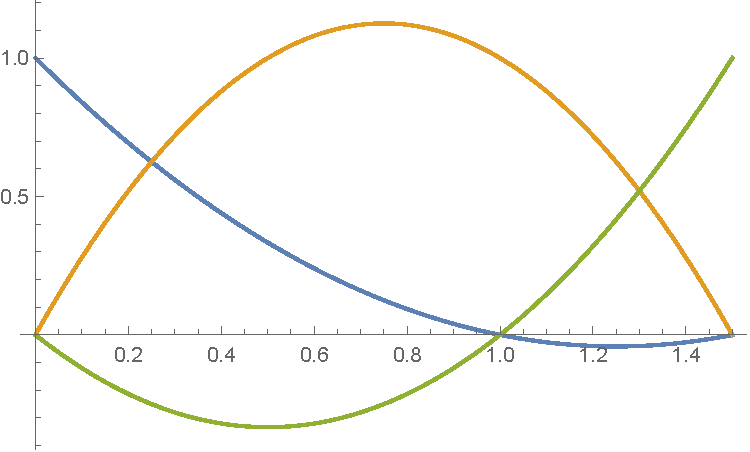
\includegraphics[width=0.8\linewidth]{img/timeBasis.pdf}
	\caption{Функции временного базиса $\eta^{m-2}(t)$, $\eta^{m-1}(t)$ и $\eta^{m}(t)$, $t_{m-2} = 0$, $t_{m-1} = 1$ и $t_{m-1} = 1.5$}
	\label{fig:timeBasis}
\end{figure}

\subsection{Тестирование на модельных задачах}
\label{hyperbolicTests}

\subsubsection{Расчётная область}

Следующие в разделе~\ref{hyperbolicTests} модельные задачи будут решены на триангуляции $\Omega_h$, построенной для квадрата $\Omega$ с вершинами $(0, \, 0)$, $(1, \, 0)$, $(1, \, 1)$ и $(0, \, 1)$ и с краевыми условиями всех типов (см. рис.~\ref{fig:modelSquare}).

\begin{figure}[!h]
	\centering
	\resizebox{0.5\textwidth}{!}{\input{img/modelSquare.pdf_tex}}
	\caption{Расчётная область $\Omega_h$}
	\label{fig:modelSquare}
\end{figure}

\subsubsection{Априорная оценка ошибки}

Известно, что численное решение~(см.~\cite[с.~124]{umea}) удовлетворяет
\begin{align}
\label{estimate}
	\normL{u(\cdot, \, t_m) - u_h(\cdot, \, t_m)} & \le
	C \, h^2 \, \Big( 
		\normL{u''_0} + \int_{t_0}^{t_l} \normL{\dot{u}''(\cdot, \, s)} \diff{s}
	\Big) \nonumber \\
	& + C \, k \, \int_{t_0}^{t_l} \normL{\ddot{u}''(\cdot, \, s)} \diff{s},
\end{align}
где $h \coloneqq$ максимальная длина ребра триангуляции $\Omega_h$. \\
Отсюда видно, что имеет место \textbf{2-й порядок сходимости по пространству и 1-й --- по времени}.

Далее мы попробуем на модельных задачах апостериорно установить порядок сходимости по времени и пространству в смысле 2--нормы.

\subsubsection{«Простая» задача}
\label{simple}

Рассмотрим сначала задачу
\begin{equation}
	2 \, \ddot{u} + \dot{u} -  \nabla^2 \, u = 2 \, (2 + t), \quad \vect{x} \in \Omega, \quad t \in \left[ 0, \, 1 \right],
\end{equation}
c краевыми условиями
\begin{align*}
	(-1, \, 0) \cdot \nabla u + u &= t^2 + x - 2 \, y - 1, \quad & \vect{x} \in \Gamma_R, & \qquad \qquad \qquad \qquad \\
	(1, \, 0) \cdot \nabla u &= 1, & \vect{x} \in \Gamma_N, & \\
	u &= t^2 + x - 2 \, y, & \vect{x} \in \Gamma_{D_1} \cup \Gamma_{D_1}, &
\end{align*}
и начальными условиями
\begin{align*}
	u(\vect{x}, 0) &= x - 2 \, y, \\
	\dot{u}(\vect{x}, 0) &= 0.
\end{align*}
Она имеет аналитическое решение $u(\vect{x}, t) = t^2 + x - 2 \, y$.

\paragraph{Решение по схеме \texttt{CN3}}

\renewcommand{\arraystretch}{2}
\begin{table}[H]
	\caption{Решение «простой»~\ref{simple} задачи по схеме \texttt{CN3}, дробление по времени}
	\label{tab:CN3plain}
	\begin{center}\begin{tabular}{|c|c|c|c|c|c|c|}
		\hline
		$h$ & $n$ & $\Delta t$ & $l$ & $\Delta_h$ & $\delta_h$ & $\frac{\delta_{2 \, h}}{\delta_h}$ \\
		\hline
		$\frac{\sqrt{2}}{6}$ & 49 & $\frac{1}{2}$ & 3 & $3.62 \times 10^{-1}$ & $5.76 \times 10^{-2}$ & \\
		\hline
		$\frac{\sqrt{2}}{6}$ & 49 & $\frac{1}{8}$ & 9 & $1.8 \times 10^{-1}$ & $2.86 \times 10^{-2}$ & 2.01 \\
		\hline
		$\frac{\sqrt{2}}{6}$ & 49 & $\frac{1}{32}$ & 33 & $4.87 \times 10^{-2}$ & $7.79 \times 10^{-3}$ & 3.67 \\
		\hline
		$\frac{\sqrt{2}}{6}$ & 49 & $\frac{1}{128}$ & 129 & $1.24 \times 10^{-2}$ & $1.99 \times 10^{-3}$ & 3.92 \\
		\hline
		$\frac{\sqrt{2}}{6}$ & 49 & $\frac{1}{512}$ & 513 & $3.11 \times 10^{-3}$ & $4.99 \times 10^{-4}$ & 3.98 \\
		\hline
	\end{tabular}\end{center}
\end{table}
\begin{table}[H]
	\caption{Решение «простой» задачи~\ref{simple} по схеме \texttt{CN3}, дробление по времени и пространству}
	\label{tab:CN3plainFull}
	\begin{center}\begin{tabular}{|c|c|c|c|c|c|c|}
		\hline
		$h$ & $n$ & $\Delta t$ & $l$ & $\Delta_h$ & $\delta_h$ & $\frac{\delta_{2 \, h}}{\delta_h}$ \\
		\hline
		$\frac{\sqrt{2}}{3}$ & 16 & $\frac{1}{2}$ & 3 & $2. \times 10^{-1}$ & $5.16 \times 10^{-2}$ & \\
		\hline
		$\frac{\sqrt{2}}{6}$ & 49 & $\frac{1}{8}$ & 9 & $1.8 \times 10^{-1}$ & $2.86 \times 10^{-2}$ & 1.8 \\
		\hline
		$\frac{\sqrt{2}}{12}$ & 169 & $\frac{1}{32}$ & 33 & $9.33 \times 10^{-2}$ & $8.45 \times 10^{-3}$ & 3.38 \\
		\hline
		$\frac{\sqrt{2}}{24}$ & 625 & $\frac{1}{128}$ & 129 & $4.65 \times 10^{-2}$ & $2.26 \times 10^{-3}$ & 3.74 \\
		\hline
		$\frac{\sqrt{2}}{48}$ & 2401 & $\frac{1}{512}$ & 513 & $2.31 \times 10^{-2}$ & $5.84 \times 10^{-4}$ & 3.88 \\
		\hline
	\end{tabular}\end{center}
\end{table}
Поясним нотации в таблицах~\ref{tab:CN3plain}~--~\ref{tab:CN3plainFull}:
\begin{itemize}
	\item $h$ --- максимальная длина ребра сетки $\Omega_h$,
	\item $n$ --- количество узлов триангуляции (размерность СЛАУ, решаемой на каждом временном слое $t_m$),
	\item $\Delta t$ --- размер шага по времени,
	\item $l$ --- количество временных слоёв,
	\item $\Delta_h \coloneqq \max_{\, 0 \le m \le l \,} \norm{\vect{u}^m - \vect{\xi}^m}_2$ --- максимальная 2-норма ошибки, \\ 
	      $\vect{u}^m \coloneqq ( u^m(\vect{x}_1), \, u^m(\vect{x}_2), \, \dots, \, u^m(\vect{x}_n) )$ --- вектор значений точного решения $u$ на $m$--м временном слое,
	\item $\delta_h \coloneqq \max_{\, 0 \le m \le l \,} \frac{\norm{\vect{u}^m - \vect{\xi}^m}_2}{\norm{\vect{u}^m}_2}$ --- максимальная относительная погрешность и 
	\item $\frac{\delta_{2 \, h}}{\delta_h}$ --- отношение предыдущей относительной погрешности к текущей.
\end{itemize}

\paragraph{Решение по схеме \texttt{BDF3}}

Решение по схеме \texttt{BDF3} сразу же при $n = 49$ и $m = 3$ (см. первую строку таблиц~\ref{tab:CN3plain}~--~\ref{tab:CN3plainFull}) даёт ошибку $\Delta_h = 3.21 \times 10^{-15}$ и относительную ошибку $\delta_h = 5.12 \times 10^{-16}$, которые сохраняются незначительными с дроблением временного шага.

\begin{figure}[!h]
	\minipage{0.45\textwidth}
	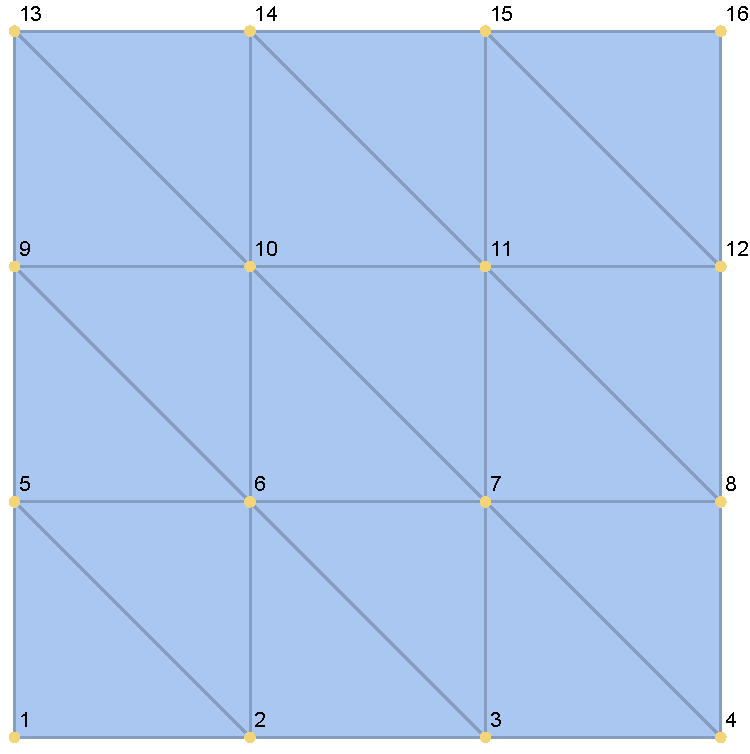
\includegraphics[width=\linewidth]{img/n16mesh.pdf}
	\caption{Сетка $\Omega_h$ из 2--й строки таблицы~\ref{tab:CN3plainFull}, $h = \frac{\sqrt{2}}{3}$ и \dots}\label{fig:n16mesh}
	\endminipage\hfill
	\minipage{0.45\textwidth}
	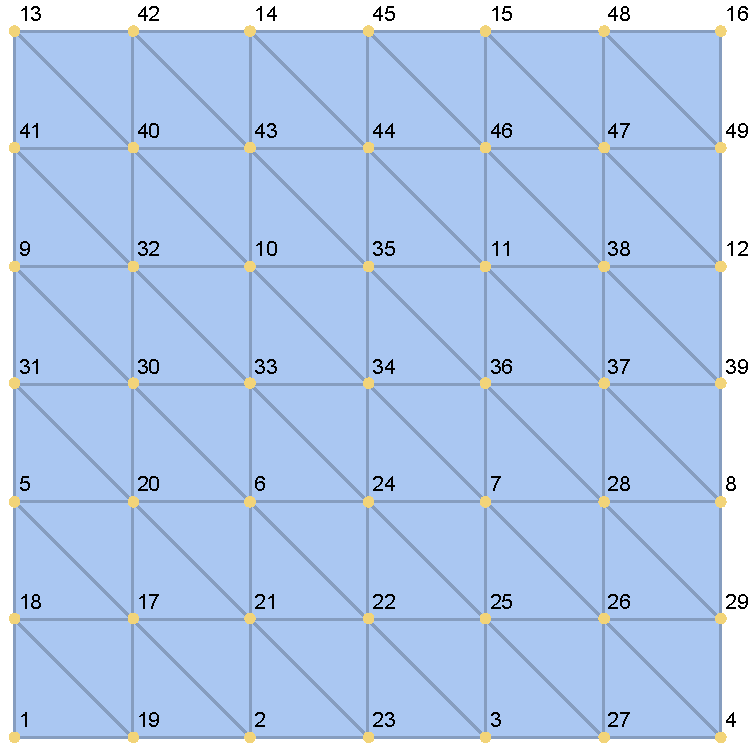
\includegraphics[width=\linewidth]{img/n49mesh.pdf}
	\caption{\dots измельчённая сетка из 3--й строки, $h = \frac{\sqrt{2}}{6}$}\label{fig:n49mesh}
	\endminipage
\end{figure}

\subsubsection{«Косинус--волна»}
\label{cosWave}

Рассмотрим теперь задачу
\begin{align*}
	& \ddot{u} + .1 \, \dot{u} -  \nabla \cdot (x \, y \, \nabla u) = \\
	& 5 \, (x + y - .1) \, \sin \big( 5 \, (t + x + y) \big) + 25 (2 \, x \, y - 1) \, \cos \big( 5 \, (t + x + y) \big), \\
	& \vect{x} \in \Omega, \quad t \in \left[ 0, \, 1 \right],
\end{align*}
c краевыми условиями
\begin{align*}
	(-1, \, 0) \cdot \nabla u + u &= 5 \, x \, y \, \sin \big( 5 \, (t + x + y) \big) + \cos \big( 5 \, (t + x + y) \big), & \vect{x} \in \Gamma_R, & \qquad \qquad \\
	(1, \, 0) \cdot \nabla u &= -5 \, x \, y \, \sin \big( 5 \, (t + x + y) \big), & \vect{x} \in \Gamma_N, & \\
	u &= \cos \big( 5 \, (t + x + y) \big), & \vect{x} \in \Gamma_{D_1} \cup \Gamma_{D_1}, &
\end{align*}
и начальными условиями
\begin{align*}
	u(\vect{x}, 0) &= \cos \big( 5 \, (x + y) \big), \\
	\dot{u}(\vect{x}, 0) &= -5 \sin \big( 5 \, (x + y) \big).
\end{align*}
Она имеет аналитическое решение $u(\vect{x}, t) = \cos \big( 5 \, (t + x + y) \big)$.

\paragraph{Решение по схеме \texttt{CN3}}

\begin{table}[H]
\caption{Решение задачи~\ref{cosWave} по схеме \texttt{CN3}, дробление по времени и пространству}
\label{tab:CN3cosWaveFull}
	\begin{center}\begin{tabular}{|c|c|c|c|c|c|c|}
		\hline
		$h$ & $n$ & $\Delta t$ & $l$ & $\Delta_h$ & $\delta_h$ & $\frac{\delta_{2 \, h}}{\delta_h}$ \\
		\hline
		$\frac{\sqrt{2}}{2}$ & 9 & $\frac{1}{2}$ & 3 & $4.15$ & $1.86$ & \\
		\hline
		$\frac{\sqrt{2}}{4}$ & 25 & $\frac{1}{8}$ & 9 & $7.4 \times 10^{-1}$ & $2.09 \times 10^{-1}$ & 8.87 \\
		\hline
		$\frac{\sqrt{2}}{8}$ & 81 & $\frac{1}{32}$ & 33 & $4.27 \times 10^{-1}$ & $6.7 \times 10^{-2}$ & 3.13 \\
		\hline
		$\frac{\sqrt{2}}{16}$ & 289 & $\frac{1}{128}$ & 129 & $2.6 \times 10^{-1}$ & $2.15 \times 10^{-2}$ & 3.11 \\
		\hline
		$\frac{\sqrt{2}}{32}$ & 1089 & $\frac{1}{512}$ & 513 & $1.36 \times 10^{-1}$ & $5.78 \times 10^{-3}$ & 3.72 \\
		\hline
	\end{tabular}\end{center}
\end{table}

\paragraph{Решение по схеме \texttt{BDF3}}

\begin{table}[H]
\caption{Решение задачи~\ref{cosWave} по схеме \texttt{BDF3}, дробление по времени и пространству}
\label{tab:BDF3cosWaveFull}
	\begin{center}\begin{tabular}{|c|c|c|c|c|c|c|}
		\hline
		$h$ & $n$ & $\Delta t$ & $l$ & $\Delta_h$ & $\delta_h$ & $\frac{\delta_{2 \, h}}{\delta_h}$ \\
		\hline
		$\frac{\sqrt{2}}{2}$ & 9 & $\frac{1}{2}$ & 3 & $2.88$ & $1.29$ & \\
		\hline
		$\frac{\sqrt{2}}{4}$ & 25 & $\frac{1}{8}$ & 9 & $4.63$ & $1.31$ & 0.985 \\
		\hline
		$\frac{\sqrt{2}}{8}$ & 81 & $\frac{1}{32}$ & 33 & $2.57$ & $4.02 \times 10^{-1}$ & 3.25 \\
		\hline
		$\frac{\sqrt{2}}{16}$ & 289 & $\frac{1}{128}$ & 129 & $1.34$ & $1.11 \times 10^{-1}$ & 3.64 \\
		\hline
		$\frac{\sqrt{2}}{32}$ & 1089 & $\frac{1}{512}$ & 513 & $6.71 \times 10^{-1}$ & $2.86 \times 10^{-2}$ & 3.87 \\
		\hline
	\end{tabular}\end{center}
\end{table}

\begin{figure}[!hb]
	\minipage{0.45\textwidth}
	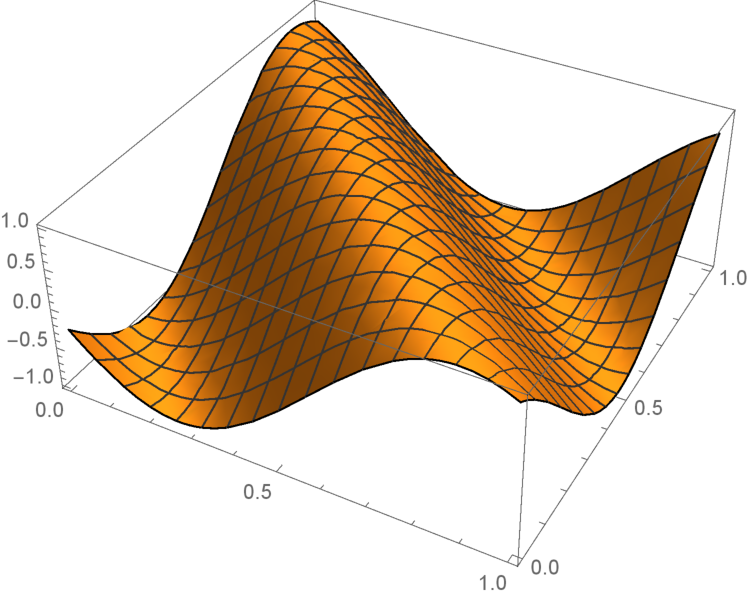
\includegraphics[width=\linewidth]{img/cosWaveAnalytic.pdf}
	\caption{Аналитическое решение $u(\vect{x}, \, .375) = \cos \big( 5 \, (.375 + x + y) \big)$ задачи~\ref{cosWave} и \dots}\label{fig:cosWaveAnalytic.pdf}
	\endminipage\hfill
	\minipage{0.45\textwidth}
	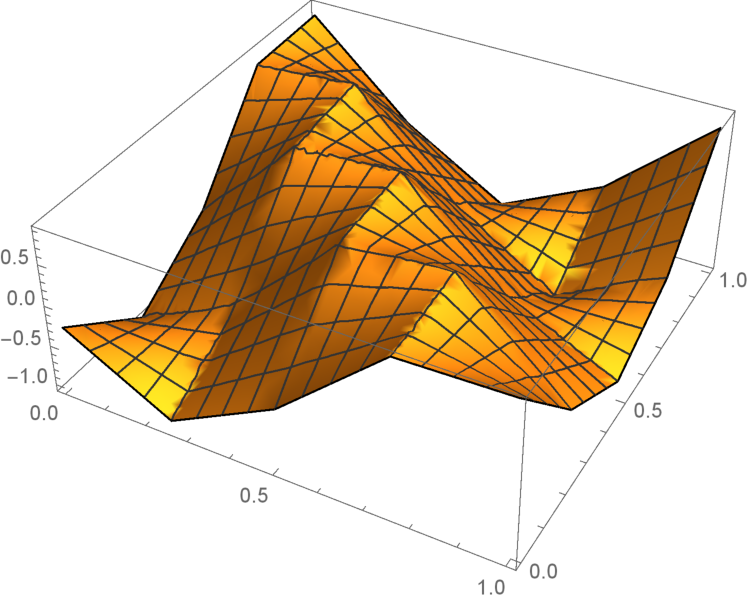
\includegraphics[width=\linewidth]{img/cosWaveNumeric.pdf}
	\caption{\dots численное решение $u_h$ на 4--м временном слое $t_4 = .375$, определённое на сетке с $n = 25$ узлами --- см. 3--ю строку таблицы~\ref{tab:CN3cosWaveFull}}\label{fig:cosWaveNumeric}
	\endminipage
\end{figure}

\subsubsection{Выводы}

Главное, на что следует обратить внимание в решениях модельных задач~\ref{simple} и~\ref{cosWave}:
\begin{itemize}
	\item Во всех таблицах (за исключением~\ref{tab:CN3plain}) видно, что мы дробим шаг по пространству $h$ в два раза, а шаг по времени $\Delta t$ --- в четыре. При этом ясно наблюдается сходимость отношения максимумов относительных погрешностей к четырём.\\
	Отсюда делаем вывод, что \textbf{численное решение $u_h$ в смысле 2-нормы сходится к аналитическому со вторым порядком по пространству и с первым --- по времени} (см. априорную оценку~(\ref{estimate})).\\
	Сходимость справедлива для обоих тестов.
	\item Очевидно, что решение задачи~\ref{simple} $u(\vect{x}, t) = t^2 + x - 2 \, y$ для любого $t$ есть житель подпространства $\mathbb{V}_h$, в котором мы ищем приближение к аналитическому решению. Стало быть нет необходимости в дроблении пространственной сетки (и, как следствие, в нагрузке на ресурсы компьютера) --- на скорость сходимости это не влияет, как видно из таблиц~\ref{tab:CN3plain} и~\ref{tab:CN3plainFull}.
	\item На «простом» тесте~\ref{simple} \texttt{CN3} сработала гораздо хуже \texttt{BDF3}, однако
	\item для уравнения с «косинус--волной»~\ref{cosWave} «усреднённые»\footnote{
			Говорят, что схемы типа Крэнка--Николсона отражают закон сохранения энергии, свойственный некоторым волновым уравнениям, не давая решению «расплываться» --- см.~\cite[с.~137]{umea}.
		} вклады от соседних временных слоёв в~(\ref{BDF3_Ab}) дали о себе знать: погрешность $\Delta_h = 1.36 \times 10^{-1}$ метода \texttt{CN3} в 5 раз меньше, чем погрешность $\Delta_h = 6.71 \times 10^{-1}$ метода \texttt{BDF3}. Более того, из таблицы~\ref{tab:BDF3cosWaveFull} видно, что только на самом мелком шаге по времени и пространству погрешность метода \texttt{BDF3} упала до второго знака;
	\item отсюда делаем вывод, что --- хотя оба метода обладают одним порядком сходимости --- скорость сходимости может очень сильно зависеть от конкретной задачи. 
\end{itemize}

\newpage
\subsection{Исходный текст программы}

Здесь мы приведём основной модуль --- пространство имён \texttt{FEMt}, содержащее решатели \texttt{CN3} и \texttt{BDF3} и вспомогательные функции для расчёта локальных матриц и векторов. Весь комплекс программ, как было отмечено в начале, доступен в репозитории:
\url{https://github.com/CATSPDEs} \\

\lstinputlisting[language=C++]{FEMt.cpp}
